\ifx\inkludert\undefined
\input{preamble}
\usepackage{xr}
\externaldocument{lin-alg}
\newcommand{\kapittel}[2]{\setcounter{chapter}{#1}\addtocounter{chapter}{-1}\chapter{#2}}
\newcommand{\kapittelslutt}{\enddocument}
\begin{document}
\chapterstyle{tma4110}
\pagestyle{plain}
\fi


\kapittel{3}{Vektorer}
\label{ch:vektorer}


\section*{To visualiseringer av et likningssystem}

I eksempel~\ref{ex:grafisk-losning} så vi at vi kunne løse systemet
\[
\systeme{
2x + 3y = 9,
-x + 6y = 3
}
\]
ved å tegne grafene til de to likningene og finne punktet der grafene
møtes:
\begin{center}
\begin{tikzpicture}[scale=.9]
\draw[->] (-1.5,0) -- (6.5,0);
\draw[->] (0,-1.5) -- (0,5.5);
\foreach \x in {-1,1,2,3,4,5,6}
\draw (\x cm,1pt) -- (\x cm,-1pt) node[anchor=north] {$\x$};
\foreach \y in {-1,1,2,3,4,5}
\draw (1pt,\y cm) -- (-1pt,\y cm) node[anchor=east] {$\y$};
\draw (-1.5,4) -- (6,-1);
\node[anchor=west] at (.4,3) {$2x + 3y = 9$};
\draw (-1.5,0.25) -- (6,1.5);
\node at (6,2) {$-x + 6y = 3$};
\filldraw (3,1) circle [radius=2pt];
\end{tikzpicture}
\end{center}

Det går også an å visualisere det samme likningssystemet på en helt
annen måte.  Vi kan si at vi gikk \emph{radvis} gjennom systemet for å
lage tegningen over: Vi så på én og én «rad» (likning) i systemet, og
tegnet grafen dens.  Men vi kan også gå gjennom systemet
\emph{kolonnevis}.  Sånn gjør vi det:

Vi ser på alle koeffisientene som står foran $x$ nedover i systemet:
$2$ og~$-1$.  Disse tenker vi på som første kolonne.  Andre kolonne
blir koeffisientene foran~$y$ (altså $3$ og~$6$), og siste kolonne
blir tallene på høyresiden (altså $9$ og~$3$).  Hver av disse
kolonnene består av to tall, og tilsvarer dermed et punkt i planet:
\begin{center}
\begin{tikzpicture}[scale=.7]
\draw[->] (-1.5,0) -- (9.5,0);
\draw[->] (0,-1.5) -- (0,6.5);
\foreach \x in {-1,1,2,3,4,5,6,7,8,9}
\draw (\x cm,1pt) -- (\x cm,-1pt) node[anchor=north] {$\x$};
\foreach \y in {-1,1,2,3,4,5,6}
\draw (1pt,\y cm) -- (-1pt,\y cm) node[anchor=east] {$\y$};
\filldraw (2,-1) circle [radius=2pt];
\node[right] at (2,-1) {$(2,-1)$};
\filldraw (3,6) circle [radius=2pt];
\node[right] at (3,6) {$(3,6)$};
\filldraw (9,3) circle [radius=2pt];
\node[left] at (9,3) {$(9,3)$};
\end{tikzpicture}
\end{center}
Hva kan vi få ut av denne tegningen?  Se på punktet $(2,-1)$, som
består av koeffisientene vi hadde foran~$x$.  Ut fra dette punktet kan
vi se hvilke verdier $x$-leddene i de to likningene kan få med
forskjellige verdier av~$x$.  Dersom $x=4$, så blir begge tallene
ganget med~$4$, og vi får $(8,-4)$.  Dersom $x=\frac{1}{2}$, så blir
begge tallene halvert, og vi får $(1,-\frac{1}{2})$.  Dersom $x=-1$,
så får vi $(-2,1)$.  Alle disse punktene ligger på en rett linje:
\begin{center}
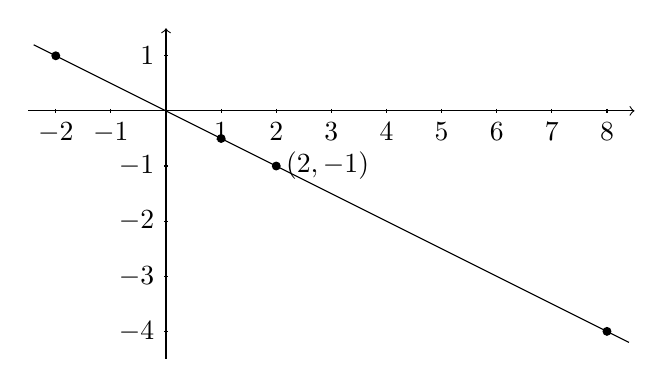
\begin{tikzpicture}[scale=.7]
\draw[->] (-2.5,0) -- (8.5,0);
\draw[->] (0,-4.5) -- (0,1.5);
\foreach \x in {-2,-1,1,2,3,4,5,6,7,8}
\draw (\x cm,1pt) -- (\x cm,-1pt) node[anchor=north] {$\x$};
\foreach \y in {-4,-3,-2,-1,1}
\draw (1pt,\y cm) -- (-1pt,\y cm) node[anchor=east] {$\y$};
\filldraw (2,-1) circle [radius=2pt];
\node[right] at (2,-1) {$(2,-1)$};
\filldraw (8,-4) circle [radius=2pt];
%\node[right] at (8,-4) {$(8,-4)$};
\filldraw (1,-.5) circle [radius=2pt];
%\node[below] at (1,-.5) {$(1,-\frac{1}{2})$};
\filldraw (-2,1) circle [radius=2pt];
%\node[above] at (-2,1) {$(-2,1)$};
\draw (-2.4,1.2) -- (8.4,-4.2);
\end{tikzpicture}
\end{center}
Denne linjen forteller oss akkurat hvilke muligheter som finnes for
$x$-leddene i de to likningene.  Vi kan velge oss et punkt på linjen
-- det tilsvarer å velge én bestemt verdi for~$x$ -- og koordinatene
til det punktet gir oss verdien av $x$-leddet i første og andre
likning.

For å gjøre det litt klarere hva som foregår her, kan vi illustrere
koeffisientkolonnen $(2,-1)$ med en pil:
\begin{center}
\begin{tikzpicture}[scale=.9]
\draw[->] (-2.5,0) -- (3.5,0);
\draw[->] (0,-1.5) -- (0,1.5);
\foreach \x in {-2,-1,1,2,3}
\draw (\x cm,1pt) -- (\x cm,-1pt) node[anchor=north] {$\x$};
\foreach \y in {-1,1}
\draw (1pt,\y cm) -- (-1pt,\y cm) node[anchor=east] {$\y$};
\draw[->] (0,0) -- (2,-1);
\node[right] at (2,-1) {$(2,-1)$};
\end{tikzpicture}
\end{center}
Når vi ganger med en $x$-verdi, så skalerer vi denne pilen opp eller
ned, uten å endre retningen dens.  Om vi for eksempel velger $x=4$, så
får vi en pil som peker i samme retning, men er fire ganger så lang.

La oss tegne piler for begge koeffisientkolonnene:
\begin{center}
\begin{tikzpicture}[scale=.7]
\draw[->] (-1.5,0) -- (9.5,0);
\draw[->] (0,-1.5) -- (0,6.5);
\foreach \x in {-1,1,2,3,4,5,6,7,8,9}
\draw (\x cm,1pt) -- (\x cm,-1pt) node[anchor=north] {$\x$};
\foreach \y in {-1,1,2,3,4,5,6}
\draw (1pt,\y cm) -- (-1pt,\y cm) node[anchor=east] {$\y$};
\draw[->] (0,0) -- (2,-1);
\node[right] at (2,-1) {$(2,-1)$};
\draw[->] (0,0) -- (3,6);
\node[right] at (3,6) {$(3,6)$};
\filldraw (9,3) circle [radius=2pt];
\node[left] at (9,3) {$(9,3)$};
\end{tikzpicture}
\end{center}
Nå kan vi spørre: Går det an å skalere opp de to pilene med hvert sitt
tall ($x$ og~$y$), slik at hvis vi følger først den ene pilen og
deretter den andre, så havner vi i punktet $(9,3)$?

Dette høres kanskje litt underlig ut, så la oss med en gang se på hva
vi får ved å putte inn tallene som vi vet er en løsning av likningen,
nemlig $x=3$ og~$y=1$.  Da gjør vi den ene pilen tre ganger så lang,
og beholder den andre som den er:
\begin{center}
\begin{tikzpicture}[scale=.7]
\draw[->] (-1.5,0) -- (9.5,0);
\draw[->] (0,-1.5) -- (0,6.5);
\foreach \x in {-1,1,2,3,4,5,6,7,8,9}
\draw (\x cm,1pt) -- (\x cm,-1pt) node[anchor=north] {$\x$};
\foreach \y in {-1,1,2,3,4,5,6}
\draw (1pt,\y cm) -- (-1pt,\y cm) node[anchor=east] {$\y$};
% \draw[->] (0,0) -- (2,-1);
% \node[right] at (2,-1) {$(2,-1)$};
\draw[->] (0,0) -- (6,-3);
\node[right] at (6,-3) {$(6,-3)$};
\draw[->] (0,0) -- (3,6);
\node[right] at (3,6) {$(3,6)$};
%\draw[->] (6,-3) -- (9,3);
\filldraw (9,3) circle [radius=2pt];
\node[left] at (9,3) {$(9,3)$};
\end{tikzpicture}
\end{center}
For å følge først den ene pilen og så den andre, flytter vi en av
pilene så den starter der den andre slutter:
\begin{center}
\begin{tikzpicture}[scale=.7]
\draw[->] (-1.5,0) -- (9.5,0);
\draw[->] (0,-1.5) -- (0,6.5);
\foreach \x in {-1,1,2,3,4,5,6,7,8,9}
\draw (\x cm,1pt) -- (\x cm,-1pt) node[anchor=north] {$\x$};
\foreach \y in {-1,1,2,3,4,5,6}
\draw (1pt,\y cm) -- (-1pt,\y cm) node[anchor=east] {$\y$};
% \draw[->] (0,0) -- (2,-1);
% \node[right] at (2,-1) {$(2,-1)$};
\draw[->] (0,0) -- (6,-3);
%\node[right] at (6,-3) {$(6,-3)$};
% \draw[->] (0,0) -- (3,6);
% \node[right] at (3,6) {$(3,6)$};
\draw[->] (6,-3) -- (9,3);
\filldraw (9,3) circle [radius=2pt];
\node[left] at (9,3) {$(9,3)$};
\end{tikzpicture}
\end{center}
Og da kommer vi til punktet $(9,3)$, som altså svarer til tallene på
høyresiden av likningene.

En fin ting med denne visualiseringen er at de to pilene vi tegnet
forteller oss noe om det som foregår på venstresiden i
likningssystemet.  Vi kan tillate oss å midlertidig ignorere
høyresiden av likningssystemet, dersom vi ønsker det.  Dermed kan vi
ta for oss spørsmål som: Hvilke andre tall kunne vi hatt på høyresiden
og fremdeles fått et løsbart likningssystem?  Er likningssystemet
løsbart uansett hvilke tall som står på høyresiden?

Om vi sammenligner denne visualiseringen av likningssystemet med den
vi så på helt først -- der vi tegnet grafene til de to likningene --
så ser vi at de ser totalt forskjellige ut.  Og disse to måtene å
tegne det på viser frem likningssystemet fra to helt forskjellige
perspektiver.

Når vi tegner grafer, så ser vi hver likning som en egen del av
tegningen.  Da er det lett å tenke på spørsmål som: Hva skjer hvis vi
tar vekk en likning?  Hva skjer hvis vi legger til en likning til?
Hva skjer hvis vi bytter ut denne likningen med en annen?




\kapittelslutt
